\documentclass{article}
\usepackage{subfigure}
\usepackage{todonotes}
\usepackage{times,amsmath,epsfig}
\title{Thesis\\ Responses to Reviewers' Comments}
\begin{document}
\maketitle

\section*{Reviewer 1}

\begin{quote}
\emph{There are some minor typo errors and some suggestions to improve some phrasings, indicated in various parts of the report, for the candidate to revise his thesis.}
\end{quote}
Thank you for reading this thesis so carefully and providing these constructive review comments, which we have accepted and amended upon in full, as described below. 

\begin{quote}
\emph{1. In chapter 2, to include a constellation diagram of an ideal OFDM received signals, such that it can be used to comparatively illustrate the effects of STO and CFO shown in Figure 2.7, 2.9, 2.10 and 2.11.}
\end{quote} 
The mentioned Figures are amended to include the constellation diagram of an ideal OFDM received signals.
%We have revised and clarified these points in the introduction section.

\begin{quote}
\emph{2. In chapter 4, how are the frame detection threshold values for various channels derived/ determined?}
\end{quote}
The threshold value depends on the operating channel and needs to be determined empirically by simulation (in common with other systems such as [36]). Assuming the set of various channels are known, the threshold for these channels can be pre-determined by simulation. The performance of synchronisation is evaluated with increased threshold within a given channel model. The threshold value corresponding to the best performance is selected for the channel model. The determined values of threshold are stored in a look-up table. Based upon the current channel model and conditions, the corresponding threshold has been selected from the look-up table. 
The discussion on determining the frame detection threshold is amended in the subsection 4.3.1 to reflect this explanation.

\begin{quote}
\emph{3. In chapter 6, figures comparing the different spectrums (e.g. 6.2, 6.3, 6.4) should be presented in different colors for clarity in comparing their characteristics.}
\end{quote}
These mentioned Figures in chapter 6 have been improved by using different colours to enhance their clarity.

\begin{quote}
\emph{4. A page listing the various notations used in the thesis should be included for easy reference when reading the thesis.}
\end{quote}
The list of notations is presented in the amended thesis at page xiv.

\begin{quote}
\emph{5. One issue that the candidate should further address in the thesis is to present results that demonstrate the practical feasibility of, as well as the real-time performance achievable by the proposed techniques when implanted on actual FPGAs. While there is no reason to doubt that functionality of the proposed techniques, it would be more convincing by developing a prototype on a FPGA device to demonstrate the correctness and real-time performance. In addition, this will also help to cross-check and compare against the results obtained through simulations, as well as provide an indication of the real-time performance achievable, which is importance for CR application. This investigation should at least be performed for the proposed receiver, and can be done based on Figure 7.1, where an 'transmitter' is synthesized to emit baseband digital data (with effects simulating the various conditions encountered under practical environment such as multipath, CFO, STO effects) that loopback to the receiver that contains the various modules. The required FPGA development resources are readily available in the research centre in NTU/SCE, and should be relatively easy to be done as the candidate had already used the relevant tools to analyse and validate individually the various proposed modules.}
\end{quote}

Each of the methods has been implemented using the FPGA development tools in a modular fashion. It means that the implemented logic was used to process captured data, and then the output from the module under test was itself captured. The output set of captured data was then presented to the next module under test. The tests were on implemented Verilog (not just on the simulated Verily). Because we have many alternative modules for most positions in the processing chain (where each one depends upon actual protocols and channels being used), it would be exhaustive and virtually impossible to test all combinations under all test scenarios, and thus the validation follows the unit test paradigm.
In fact a carefully-designed test-bench has been generated for every module, following industry standard practices for FPGA development.
Furthermore, the captured data streams were cross-compared with a MATLAB simulation to ensure correctness. In other words, the output of a module is compared to the MATLAB simulation output for that module. This data then forms the input of the next module (who's output is also checked against the MATLAB data).

Regarding real-time effects, chapter 7 analyses the ability of a proposed architecture applied the proposed method for a multiple standard application with regard to the adaptive time when system switches from one standard to another. %As can be seen in Fig. 7.1, building up a prototype for demonstration requires a lot of hard engineering works.

Please note also that a prototype CR implementation is beyond the scope of this work (and requires a lot of practical issues to be solved, as well as having a working CR engine, RF or IF digital front-end, and MCMM. 

To be clear, the main contributions of this thesis are to propose novel techniques to overcome the well-known practical issues of OFDM for multiple standard CR application, such as synchronisation and spectral leakage. %The proposed methods are implemented by using Verilog HDL. The verification for the implementation is intensively done by the test-benches in which the output and intermediate values are compared to that of Matlab simulation to evaluate the correctness. 
Further works for verifying a system integration framework making use of these techniques are described in a new sub-section 7.5 in Chapter 7. This totally new sub-section presents comprehensive system verification results from test-benches performed on Xilinx tools, and compares this to the performance of a `golden model' simulated in MATLAB.


\section*{Reviewer 2}
\begin{quote}
\emph{While this work relates to cognitive radio applications, the decision making aspects of cognitive radio are not addressed in this dissertation, which is fine. Perhaps this should be made clear in the introduction.}
\end{quote}
First of all, thank you for your review. I have amended the text exactly as requested in the comments.
This point is clearly revised in the introduction.

\begin{quote}
\emph{1. In Section 2.1, Mr. Pham states that “… OFDM system implementation is simple, low cost, and can be more effectively parameterized than FBMC systems.” Further justification of this assertion is needed. It may be helpful to provide a more comprehensive comparison between OFDM and FBMC techniques.}
\end{quote}
This point was amended in the subsection 2.1.1 to provide more comprehensive comparison between OFDM and FBMC described as follows:
In order to understand FBMC and its distinctness from OFDM, it is best to study multicarrier systems, in which the output signal can be expressed in the continuous time domain as Equ.\ref{equ:multicarriermodulation}. 
This can be a unified formulation for both OFDM and FBMC.
\begin{eqnarray}
\label{equ:multicarriermodulation}
s(t) = \sum_{n}\sum_{k  = 0}^{N-1} x_{k}[n] h(t-nT)e^{i2\pi (t-nT)f_{k}},
\end{eqnarray}	
where $x_{k}[n]$ denotes the sample of the $k_{th}$ subcarrier data symbol in $n_{th}$ symbol of continuous multicarrier symbols, $f_{k}$ is the $k_{th}$ subcarrier in a set of $N$ used subcarriers, $T$ is the multicarrier symbol duration, and $h(t)$ is a prototype filter.
\begin{figure}[b]
	\centerline{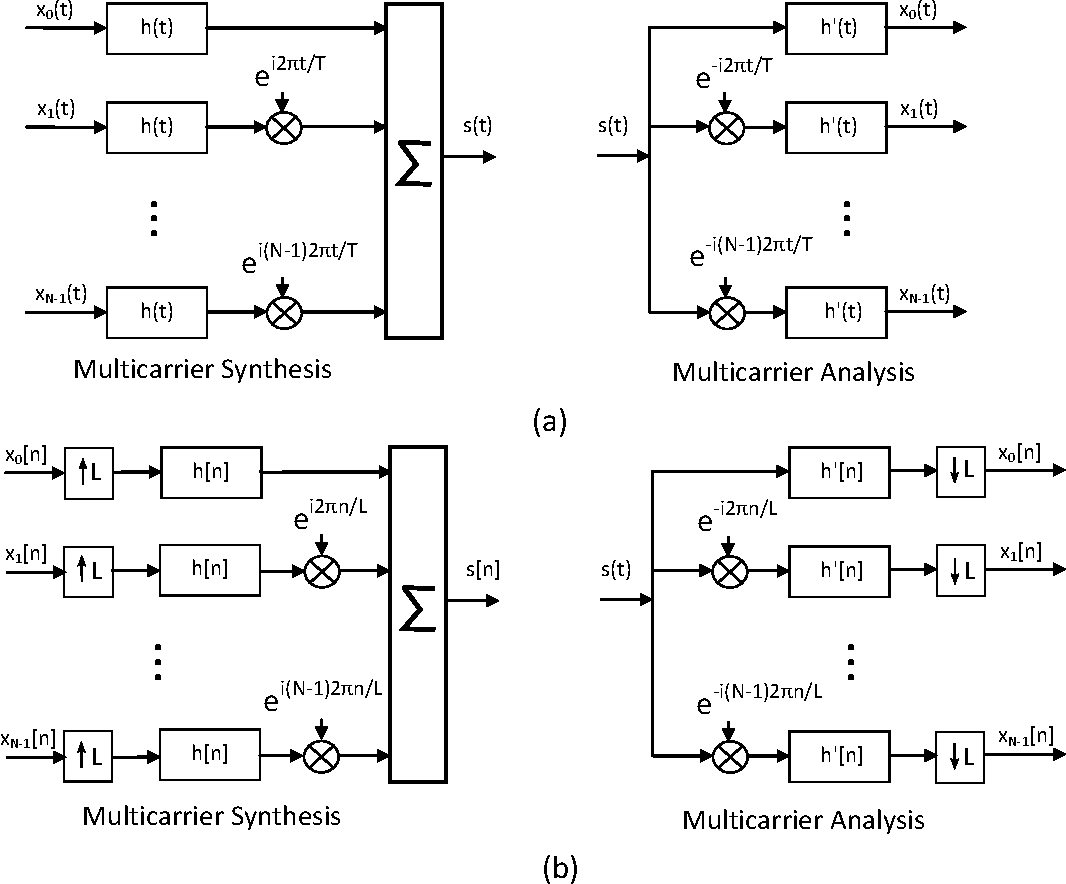
\includegraphics [width=0.8\columnwidth] {../Figures/multucarrier_system} }
	\caption{Block diagram of a multicarrier modulated system, (a) in the countinuous-time and (b) in discrete-time}
	\label{fig:multicarrier-block}
\end{figure}
This transceiver of multicarrier system can be modelled as a block diagram, shown in Fig.~\ref{fig:multicarrier-block}.
As can be seen in the discrete-time domain, $N$ data symbols at synthesis are up sampled by a factor of $L$, which is calculated by $\frac{T}{T_{S}}$, $T_{S}$ denotes sample period of output sequence $s[n]$, and then filtered by a prototype filter $h[n]$. The output of each data stream will be modulated by frequency of multi-carriers and the summed for transmission. 
The signal in the receiver is demodulated and then filtered by a bank of matched filters $h'[n]$, and down sampled by a factor of $L$. 
When critical sampling applies, $L = N$ and the prototype filter $h[n]$ is selected as a rectangular pulse in the time domain, i.e. a $sinc$ pulse in the frequency, this multicarrier system becomes a conventional OFDM system.

FBMC is different from OFDM in the selection of the prototype filters $h[n]$, and matched filters $h'[n]$. Also, the $h[n]$ and $h'[n]$ filters are chosen and designed depending on the adopted FBMC modulation technique.
By using the well-designed filters for each subcarrier, FBMC could be a more effective solution in comparison to OFDM in term of ICI cancelation and spectral leakage suppression because nonadjacent subcarriers are almost completely separated by a bank of filters. 

On the other hand, OFDM has been the dominant technique adopted for broadband multicarrier communication.
OFDM has many important and desirable features over the FBMC. OFDM was originally developed focusing on a low-complexity implementation. The low complexity of OFDM is achieved thanks to a fundamental assumption in which subcarriers of OFDM symbol are perfectly synchronized and orthogonal with the consecutive subcarriers. Thus the subcarriers are used for modulation at the transmitter using an IFFT block; inversely, they are separated by using an FFT block at the receiver. By contrast, FBMC may be more complex than OFDM. The demand for well-designed filters in FBMC results in increasing complexity and resource requirements. Moreover, while employing MIMO technique in OFDM to increase the system's capacity and resulting in high spectral efficiency is a straightforward work, unfortunately, the development of MIMO-FBMC systems is relatively more complex.
OFDM modulation has been the dominant technique adopted for many wireless standards and has been investigated in terms of spectral sensing and carrier allocation for CRs.
OFDM system implementation is simple, low cost, and can be more effectively parameterised.
A single baseband implementation can be made to flexibly support multiple standards like 802.11[14], 802.16[15], and 802.22[16], as well as supporting future OFDM-based standards.

\begin{quote}
\emph{2. Chapter 3 presents the multiplierless correlator work. There are aspects of this chapter that may need further examination. I appreciate the significance of the problem this chapter is addressing, and the value in the demonstrated savings; however, the methods for performing the comparisons don't always seem fair.
One note in resource usage: a DSP48 processing module is rated to operate at hundreds of MHz. If the desired operation speed is N times slower than the maximum operating speed, then a single DSP48 can cover N instances of the operation through time multiplexing. Therefore, when performing a resource estimate, the required number of units should be derated by the operational speed, otherwise it represents an underutilized system. In this case, the target operating frequency is 50 MHz while capacity of the DSP48s are over 300 MHz.	}
\end{quote}
The additional discussion on the aspect of operating speed is added as follows:  
``The multiplierless correlator and the DSP-based correlator can operate at a speed which is multiple times higher than the desired operating speed for baseband modulation. Both of them can therefore make use of time multiplexing to obtain a trade-off between resource usage and operating speed. However, it should be noted that increased operating speed leads to significantly increased power since the power consumption is proportional to the square of operating speed. To provide a fair comparison, both the multiplierless correlator and the DSP-based correlator are investigated on the same transposed direction form.''
The text in subsection 3.2.3 has been amended to include this point.  But it should be noted that the structure of time multiplexing within the correlator is a potentially extensive research area in its own right, and is beyond the scope of the current investigation.'


\begin{quote}
\emph{3. While power comparisons are made between the multiplierless version and DSP48 version, it isn’t clear if the same highly quantized coefficients are being used in the DSP48 case. If not, I would expect those values to drop significantly. To a degree, this discussion breaks down into a traditional precision analysis problem. If indeed 32 bits of precision are not needed in this correlator, then the DSP48 could be the wrong component to use.}
\end{quote}
The use of a DSP48-based implementation when comparing to the multiplierless version is further discussed as follows:
``To obtain a precise computation, the DSP48 is typically used for multiplication in fixed point format, Q1.15. Because the DSP48 is a hardcore, it is impossible to optimise the internal components of DSP48 in the case of reducing the number of bits used in the computation. The static power of the DSP based correlator will then not drop significantly when reducing the number of bits in the words being computed. Thus the use of DSP48 for calculation of words with fewer bits is wasteful as well as having reduced precision. Hence, it is not necessary to evaluate the DSP48 version when comparing a system that employs just a small number of  bits for computation.''
This explanation is added in the chapter 3 at the subsection 3.2.3.

\begin{quote}
\emph{4. It states that the multiplierless design must be specified manually, and cannot be inferred by the tools from higher level descriptions (I assume HDLs). After reviewing the structure presented in this chapter, I believe this assertion should be reexamnied.}
\end{quote}
This assertion has been revised to clarify the discusson as follows:
``The correlator designs must be specified manually, and cannot be inferred by the tools from higher level descriptions such as high level synthesis (HLS) or Simulink that allows designing system at high level abstraction.''
This amendment is made in the chapter 3 at the section 3.2.

\begin{quote}
\emph{5. Taking advantage of the periodic nature of the energy distribution is an excellent way of reducing the computational burden of gross frame synchronization. When compared to full cross-correlation techniques this reduces the needed computation to a much smaller viable amount.}
\end{quote}
The computational reduction is further explained to show clearly how it achieves a significant decrease in terms of resource usage as follows: 
``The needed computation of the proposed architecture for frame synchronization compared to the use of a full cross-correlation technique is minimised by not only taking advantage of the periodic nature of the preamble. 
It should be noted that profiting from the real number computation of the proposed metrics, instead of requiring complex computations, and from using a multiplierless correlator, also yield a significant computational saving.''
This amendment is made in the chapter 4 at the subsection 4.3.4.2.

\begin{quote}
\emph{6. In Chapter 6, the performance of the proposed solution is very good, but seems to come at a significant computational cost due to the extension of the IFFT and increased sample rate. These costs should be quantified.}
\end{quote}
The discussion on computational cost is extended by providing a additional complexity analysis in terms of hardware usage (i.e. FFs and DSPs) for dynamically sized IFFT blocks and the FIR filter. This amendment is made in the chapter 6 at the subsection 6.4.2.

\begin{quote}
\emph{7. In Chapter 7, the premise is that faster reconfiguration is better, yet very little is provided on the requirements for when it is fast enough. There is significant emphasis on buffering streams at the boundaries of PR modules. I can appreciate the object of not wanting drop any data; however, for the radio standards discussed in previous chapters, there are higher-level protocols that manage the retransmission of lost or dropped packet of data.}
\end{quote}
I accept your point that higher layers can potentially handle the lost data, however it is good practice to prevent, or at least minimise, data loss in lower layers -- this is because of the tendency for lower-layer data loss to have more serious knock-on effects at higher layers (i.e. the  loss magnification when climbing the layer stack). This point is now discussed in more detail within the revised thesis as follows:
``When the system adapts to a new condition (i.e., switching the operating standard), a reconfiguration operation is performed which may pause or suspend data processing for the duration of the reconfiguration. Received packets of data may therefore be lost. 
The reconfiguration is required to operate fast enough that the input data buffered during reconfiguration does not overflow the buffer, leading to entire packets of data being dropped. Even though there are higher-level protocols available to manage the retransmission of lost or dropped packet of data, performing these mechanisms is wasteful and may significantly increase the cost in terms of computation and power consumption.''
This amendment is made in the chapter 7 at the section 7.1.

\begin{quote}
\emph{8. One other issue with this chapter is that Mr. Pham is allowing the limitations of the tool establish bounds on what is possible with this work, instead of examining the theoretical limits of FPGA re-programmability. Much of this is due to the acceptance of the slot-based partial reconfiguration (PR) module. This, in turn, skews some of the metrics used throughout the chapter. For example, Table 7.4 summarizes the resource usage of several radio components. Since the PR slot model is assumed, all of the resource in the slot are consumed by the component, regardless of whether they are used in the computation or not. The configuration time for a component of a given slot is constant, even if it small component (an impact on the reconfiguration latency – a metric used in this chapter).}
\end{quote}
Chapter 7 focuses on the OFDM-based CR architecture to reduce the reconfiguration time by applying PR technique and parameterised modules which come into play when the system is adapted. Fundamental research on PR methods is out of scope of this thesis. However, the aspect of PR methods is worth being mentioned. This point is therefore further discussed in the revised thesis as follows:
``Because slot based PR is widely used as well as being supported by Xilinx tools, we assume that slot-based PR is employed for performing PR.
All of the resources in the slot are consumed by the component, regardless of whether they are used in the computation or not. The configuration time for a component of a given slot is thus also constant, even if it small component.
There is some research [a1] on reducing the wasted resources from unused logic in PR slots for small components that may reduce the reconfiguration time of such components. However, these approaches are just for limited FPGA devises, and require substantially more expert work to implement the designs.  
Furthermore, this improvement still does not help the overall reconfiguration latency because the overall latency has to take into account the worst case latency (i.e., the reconfiguration time of the largest components) when the system adapts from a standard to another.''
This amendment is made in the chapter 7 at the section 7.4.2.
[a1]  Sohanghpurwala, A.A.; Athanas, P.; Frangieh, T.; Wood, A., "OpenPR: An Open-Source Partial-Reconfiguration Toolkit for Xilinx FPGAs," IEEE International Symposium on Parallel and Distributed Processing Workshops and Phd Forum (IPDPSW), May 2011

\begin{quote}
\emph{9. The strategy of over-clocking a component immediately after it has been reconfigured to clear the backlog, the turn to normal clocking speed has consequences: designing a module to operate at 2x the needed clock rate is likely going to consume more resources than a component optimized for 1x clock speed.}
\end{quote}
The strategy of over-clocking is explained more clearly as follows:
``Increasing operating speed is done basically by controlling the MMCM module to adjust the speed of the input clock of the receiving modules, rx\_clk. Because these modules implemented on FPGA fabric are able to work with a clock that is higher than 2X the operating clock, designing these modules to support twice the normal operating clock does not consume more resources compared to the case of the normal clock speed.''
This amendment has been added into chapter 7 at the subsection 7.3.1.\newline



I would like to thank the reviewers for their insightful comments that have helped improve the thesis.

\end{document}
